\documentclass[11pt]{article}
\usepackage{fullpage,url}
\usepackage{amsmath,amsthm,amssymb}
\usepackage{graphicx}
\usepackage{eso-pic}
\usepackage{bm}
\usepackage{caption}
\usepackage{picins}   
\usepackage{microtype}
\usepackage{multirow}
\usepackage{url}
\usepackage{enumerate}
\usepackage{pdfpages}
\usepackage[letterpaper,top=1in,bottom=1in,left=1in,right=1in,nohead]{geometry}

\newcommand{\PhiB}{\mathbf{\Phi}}
\newcommand{\Ll}{\mathcal{L}}
\newcommand{\Nn}{\mathcal{N}}
\newcommand{\Uu}{\mathcal{U}}
\newcommand{\Ee}{\mathcal{E}}
\newcommand{\Aa}{\mathcal{A}}
\newcommand{\Hh}{\mathcal{H}}
\newcommand{\Ii}{\mathcal{I}}
\newcommand{\Ff}{\mathcal{F}}
\newcommand{\Dd}{\mathcal{D}}
\newcommand{\Tt}{\mathcal{T}}
\newcommand{\Pp}{\mathcal{P}}
\newcommand{\Ss}{\mathcal{S}}
\newcommand{\Cc}{\mathcal{C}}
\newcommand{\Oo}{\mathcal{O}}
\newcommand{\Bb}{\mathcal{B}}
\newcommand{\Rr}{\mathcal{R}}
\newcommand{\Rm}{\mathrm{R}}
\newcommand{\CB}{\mathbf{C}}
\newcommand{\RB}{\mathbf{R}}
\newcommand{\xB}{\mathbf{x}}
\newcommand{\yB}{\mathbf{y}}
\newcommand{\XB}{\mathbf{X}}
\newcommand{\YB}{\mathbf{Y}}
\newcommand{\fB}{\mathbf{f}}
\newcommand{\ZB}{\mathbf{Z}}
\newcommand{\SB}{\mathbf{S}}
\newcommand{\AB}{\mathbf{A}}
\newcommand{\WB}{\mathbf{W}}
\newcommand{\TB}{\mathbf{T}}

\newcommand{\omitme}[1]{}
\newtheorem*{lemma}{Lemma}
\newtheorem{case}{Case}

\makeatletter
\newcommand{\specialnumber}[1]{%
  \def\tagform@##1{\maketag@@@{(\ignorespaces##1\unskip\@@italiccorr#1)}}%
}

\setlength{\parindent}{0in}
\setlength{\parskip}{6pt}

\DeclareMathOperator{\E}{E}
\DeclareMathOperator{\Var}{Var}
\DeclareMathOperator{\Unif}{Unif}

\begin{document}
\thispagestyle{empty}
{\large{\bf CS6957: Probabilistic Modeling \hfill Prateep Mukherjee(u0876583)}}\\

{\LARGE{\bf Homework 4}}
\vspace{0.2\baselineskip}
\hrule

\par 1. \textbf{\large{NOTE: Please see program p1.r for this question.}}

\vspace{-5pt}

\begin{figure}[hbt!]
\centering
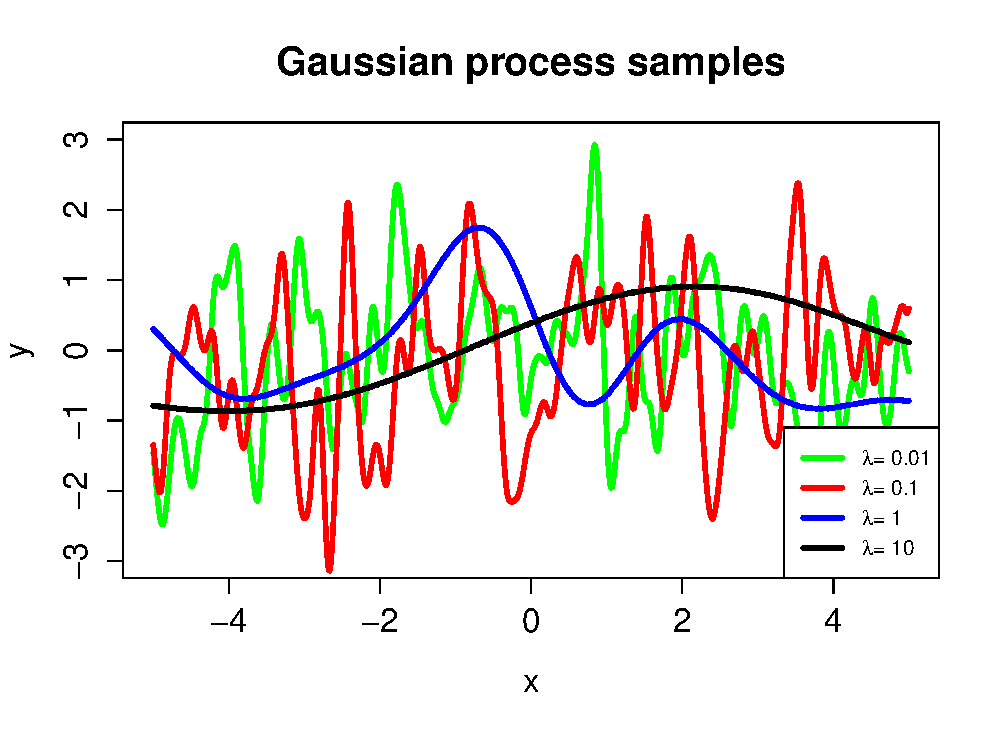
\includegraphics[width=0.8\linewidth]{p1.pdf}
\vspace{-25pt}
\caption{Gaussian process regression functions for different $\lambda$ values}
\label{fig1}
\end{figure}

%\vspace{-10pt}

\par 2 \textbf{\large{NOTE: Please see program p2.r for this question.}}

\vspace{-10pt}

\begin{figure}[hbt!]
\centering
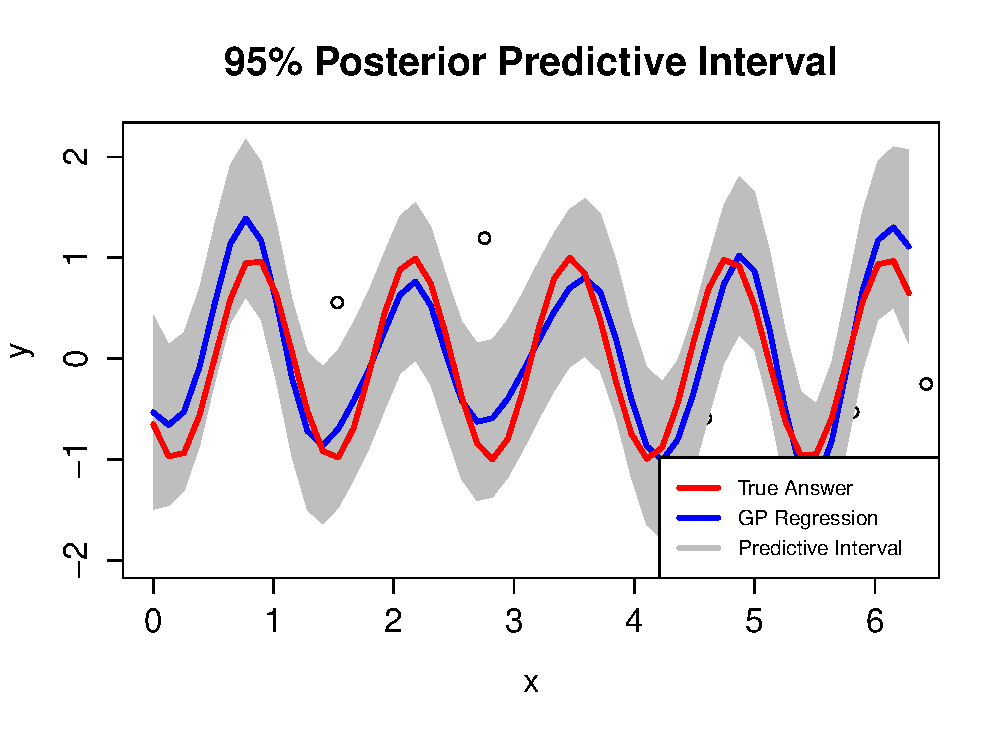
\includegraphics[width=0.8\linewidth]{p2.pdf}
\vspace{-25pt}
\caption{GP regression and true values plotted. $\lambda=1.5$}
\label{fig2}
\end{figure}

\par 3 \textbf{\large{NOTE: Please see program p3.r for this question.}}

\vspace{-10pt}

\begin{figure}[hbt!]
\centering
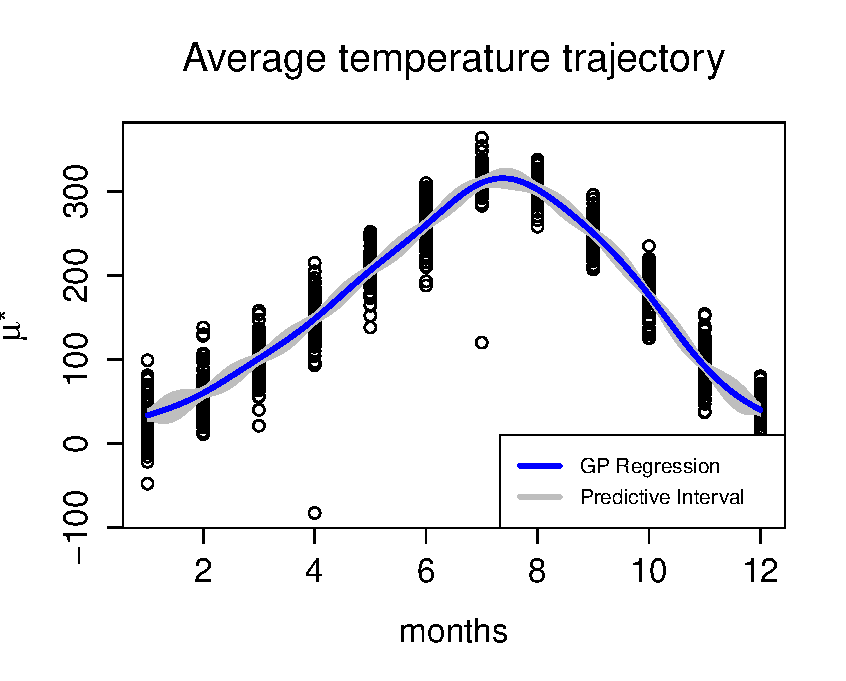
\includegraphics[width=0.8\linewidth]{p3a.pdf}
\vspace{-25pt}
\caption{Average cyclical temperature over the course of a year}
\label{fig3}
\end{figure}

\vspace{-20pt}

\begin{figure}[hbt!]
\centering
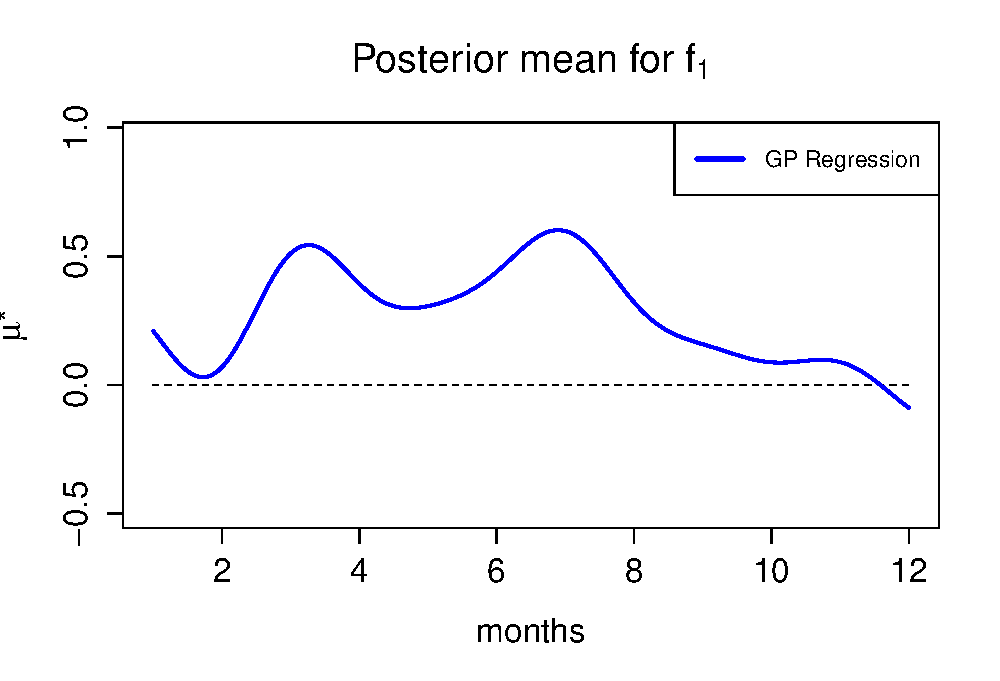
\includegraphics[width=0.8\linewidth]{p3b.pdf}
\vspace{-25pt}
\caption{Posterior mean for $f_1$ plotted over every month. Blue line shows the estimated posterior distribution }
\label{fig4}
\end{figure}

\par Fig. \ref{fig4} shows the rate of change of average daily maximum temperature for every month. The graph shows that temperatures have increased over all the months, except for December. This shows that temperatures in SLC have increased on average over the years.

\begin{figure}[!t]
\centering
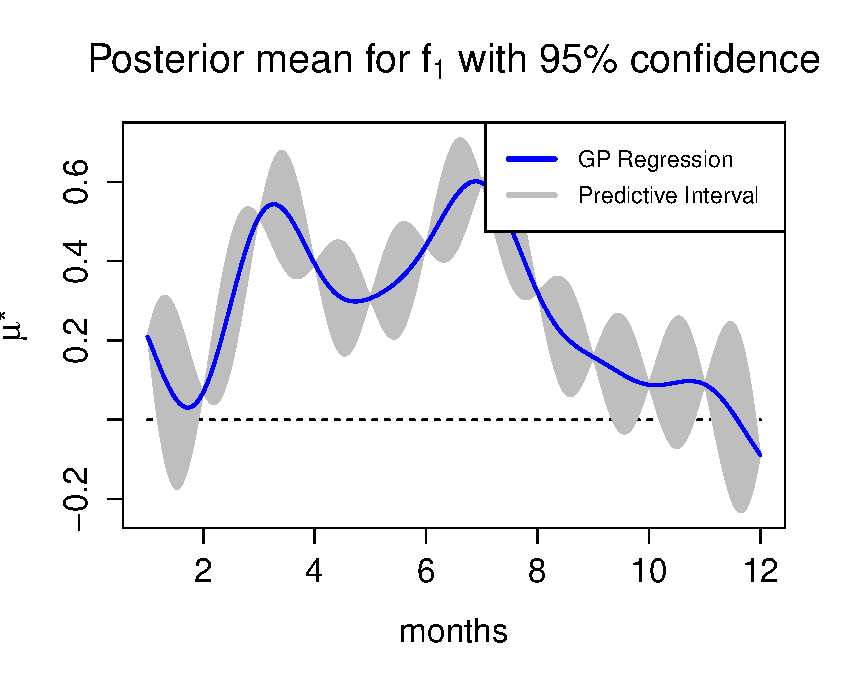
\includegraphics[width=0.7\linewidth]{p3b_1.pdf} \\
\vspace{-50pt}
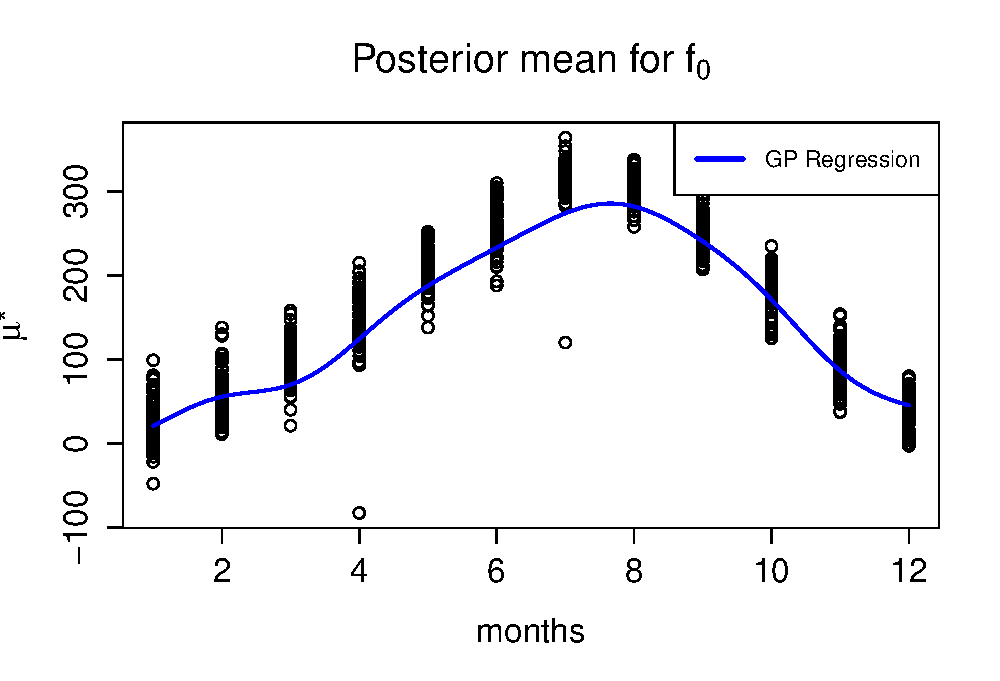
\includegraphics[width=0.7\linewidth]{p3b_0.pdf} \\
\vspace{-50pt}
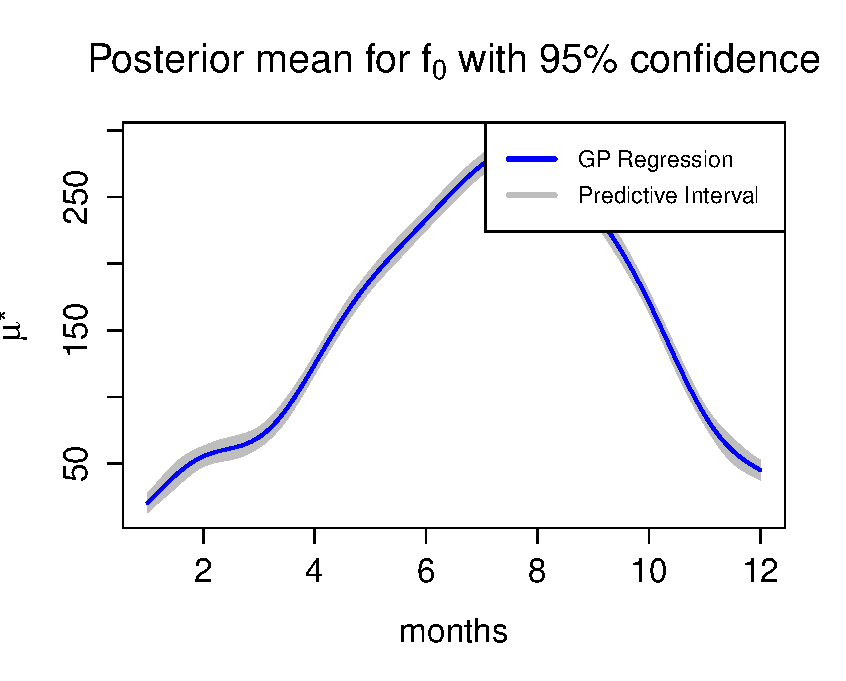
\includegraphics[width=0.7\linewidth]{p3b_0_1.pdf} \\
\vspace{-25pt}
\caption{Posterior mean for $f_1$(top) and $f_0$(center,bottom) plotted over every month. Blue line shows the estimated posterior distribution, grey shows the 95\% confidence interval. }
\label{fig5}
\end{figure}

\end{document}